%! alt Coordinate plane with the x-axis and the line y = 10. A = (0, 3) is reflected in the x-axis to A' = (0, -3), and B = (24, 5) is reflected in y = 10 to B' = (24, 15). The straight segment from A' to B', of length 30, crosses the x-axis at P = (4, 0) and the line y = 10 at Q = (52/3, 10). The highlighted path runs from A to P to Q to B.
%! after_paragraph 1
%! scale 1/5
% The shared preamble of every Cevian figure. pipeline/figures turns these colours into theme-aware paint,
% and refuses any other colour, so draw only with them:
%   figink (lines and labels), figaux (construction lines), figaccent (the object the argument turns on),
%   figtint and figaccenttint (light fills).
\documentclass[border=1.5pt]{standalone}
\usepackage{tkz-euclide}
\definecolor{figink}{RGB}{0,0,0}
\definecolor{figaux}{RGB}{85,85,85}
\definecolor{figaccent}{RGB}{192,57,43}
\definecolor{figtint}{RGB}{221,221,221}
\definecolor{figaccenttint}{RGB}{245,213,208}
% tkz-euclide's defaults draw circles, compasses and marks in 50% grey and fill points with a tint.
\makeatletter
\def\tkz@otherlinecolor{figink}
\def\tkz@euc@circlecolor{figink}
\def\tkz@euc@compasscolor{figink}
\def\tkz@euc@mkcolor{figink}
\def\tkz@mk@fill{figink}
\def\tkz@euc@pointfillcolor{figink}
\makeatother
\tkzSetUpLine[color=figink,line width=.7pt]
\tkzSetUpArc[color=figink,line width=.7pt]
\tkzSetUpCompass[color=figink,line width=.5pt]
\tkzSetUpPoint[color=figink,fill=figink,size=3.1pt]
\tikzset{
  every picture/.style={line cap=round,line join=round,color=figink},
  circle style/.append style={color=figink,line width=.7pt},
  aux/.style={color=figaux,line width=.45pt,dash pattern=on 2.6pt off 2pt},
  key/.style={color=figaccent,line width=1pt},
  mk/.style={color=figink,line width=.5pt},
  lbl/.style={color=figink,inner sep=2.2pt},
  len/.style={color=figink,inner sep=1.5pt,font=\small},
}

\begin{document}
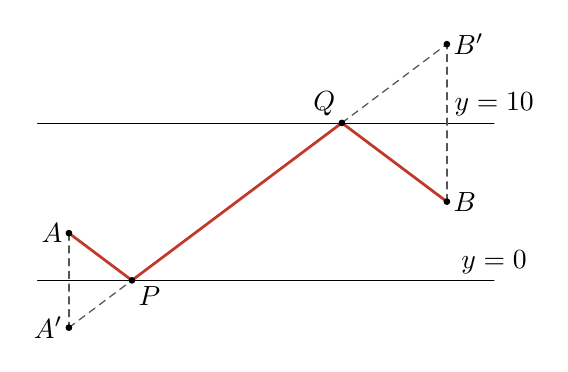
\begin{tikzpicture}
\tkzDefPoint(0.0,0.60000000){A} %! A = (0, 3)
\tkzDefPoint(4.8000000,1.0000000){B} %! B = (24, 5)
\tkzDefPoint(0.0,-0.60000000){Ap} %! Ap = (0, -3)
\tkzDefPoint(4.8000000,3.0000000){Bp} %! Bp = (24, 15)
\tkzDefPoint(0.80000000,0.0){P} %! P = (4, 0)
\tkzDefPoint(3.4666667,2.0000000){Q} %! Q = (52/3, 10)
\tkzDefPoint(-0.40000000,0.0){L} %! L = (-2, 0)
\tkzDefPoint(5.4000000,0.0){R} %! R = (27, 0)
\tkzDefPoint(-0.40000000,2.0000000){U} %! U = (-2, 10)
\tkzDefPoint(5.4000000,2.0000000){V} %! V = (27, 10)
%! fact equal(dist(A, P), dist(Ap, P))
%! fact equal(dist(Q, B), dist(Q, Bp))
%! fact collinear(P, Ap, Bp)
%! fact collinear(Q, Ap, Bp)
%! fact dist(Ap, Bp) == 30
%! fact dist(A, P) + dist(P, Q) + dist(Q, B) == 30
\tkzDrawSegment(L,R)
\tkzDrawSegment(U,V)
\tkzDrawSegments[aux](Ap,P Q,Bp A,Ap B,Bp)
\tkzDrawPolySeg[key](A,P,Q,B)
\tkzDrawPoints(A,B,Ap,Bp,P,Q)
\tkzLabelPoint[left,lbl](A){$A$}
\tkzLabelPoint[right,lbl](B){$B$}
\tkzLabelPoint[left,lbl](Ap){$A'$}
\tkzLabelPoint[right,lbl](Bp){$B'$}
\tkzLabelPoint[below right,lbl](P){$P$}
\tkzLabelPoint[above left,lbl](Q){$Q$}
\tkzLabelPoint[above,lbl](R){$y = 0$}
\tkzLabelPoint[above,lbl](V){$y = 10$}
\end{tikzpicture}
\end{document}
